\section{Практическая часть}

\subsection{Конвекция в замкнутой петле}

\begin{figure}[h]
    \centering
    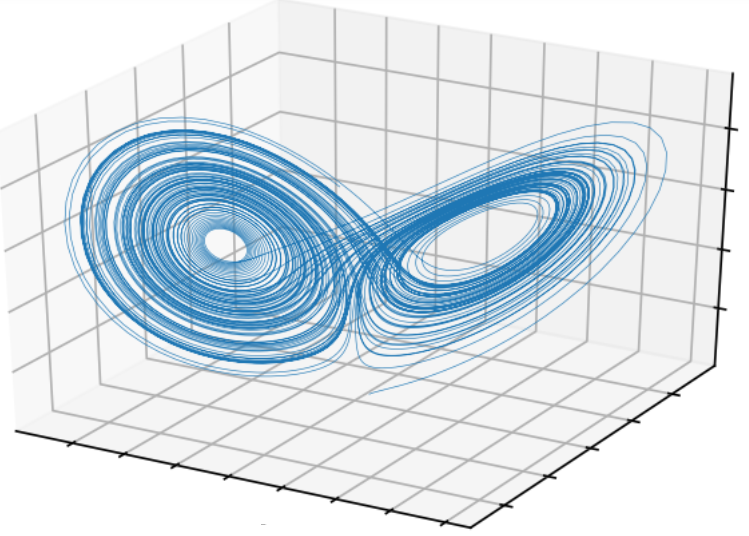
\includegraphics[width=0.5\textwidth]{img/attr_L.png}
    \caption{Визуализация численного моделирования аттрактора Лоренца (3D)}
    \label{fig:att_L}
\end{figure}

Пусть имеем замкную в кольцо (ось кольца параллельна земле) трубку, заполненную жидкостью. Трубка подогревается снизу и охлаждается сверху.
При достаточно большой интенсивности подогрева возможно возникновение конвекционного течения.угловую координату $\varphi$, отсчитываемую от направленного вниз радиуса против часовой стрелки. 
Зависимость температуры от угла $T = T(\varphi)$ имеет период $2 \pi$ и её можно представить в виде ряда Фурье, ограничимся учетом только первой гармоники: 
$$T(\varphi) = T_0(1 + Y \sin \varphi + Z \cos \varphi)$$

Из уравнения можно увидеть, что $Z$ в нашей модели отвечает за отклонение температуры от среднего значения в нижней точки трубы, $Y$ за крайние $\varphi = \pi/2$.
Через $X$ обозначим скорость течения, которая не зависит от $\varphi$ в силу несжимаемости жидкости.

Исходя из качественных соотношений составим уравнения для динамических переменных $X, Y, Z$.

Изменения скорости течения вызывается силой, которая пропорциональна $Y$, и течение тормозится силой вязкого трения, котрая пропорциональна $X$. Таким образом имеем первое уравнение: $\dot{X} = c Y - \beta X$.

Предположим, что имеет место течение с постоянной скоростью, $\dot{\varphi} = X$. Тогда можно записать:
$$T = f(\varphi - X t) = T_0(1 + Y \sin (\varphi - X t) + Z \cos(\varphi - X t))$$
Введя обозначение $\varphi' = \varphi - X t$:
$$\dot{T} = T_0(Y \dot{\varphi}' \cos \varphi' - Z \dot{\varphi}' \sin{\varphi'}) = T_0(- X Y \cos \varphi' + Z X \sin \varphi').$$

Отсюда видно, что перенос температуры потоком жидкости учитывается членом вида $X Z$ в уравнении для $Y$ и членом $(- X Y)$ в уравнении для $Z$. В оба уравнения следует добавить члены, учитывающие релаксацию, которые будут иметь вид, соответственно, $(- D Y)$ и $(- D Z)$, где $D$ -- константа, а также учесть подогрев добавлением постоянного члена $A$ в уравнение для $Z$. Итого имеем:
$$\dot{Y} = X Z - D Y, \hspace{1cm} \dot{Z} = A - X Y - D Z$$
Далее, производя замену переменных для уравнений для $X, Y, Z$:
$$X = D x, \hspace{1cm} Y = \frac{\beta D y}{c}, \hspace{1cm} Z = -\frac{\beta D z}{c}, \hspace{1cm} t = D t,$$
получаем уравнения Лоренца:
\begin{equation}
    \label{LL}
\boxed{\dot{x} = \sigma(y-x), \hspace{1cm} \dot{y} = r x - y -x z, \hspace{1cm} \dot{z} = -b z + x y}
\end{equation}
где $\sigma = \frac{\beta}{D}$, $r = \frac{c A}{\beta D^2}$, $b =1$. 

Система \eqref{LL} была числено решена в \textit{Python}. Данные визуализации представлены на рис. \ref{fig:att_L} и рис. \ref{fig:xyz}.

\begin{figure}
    \centering
    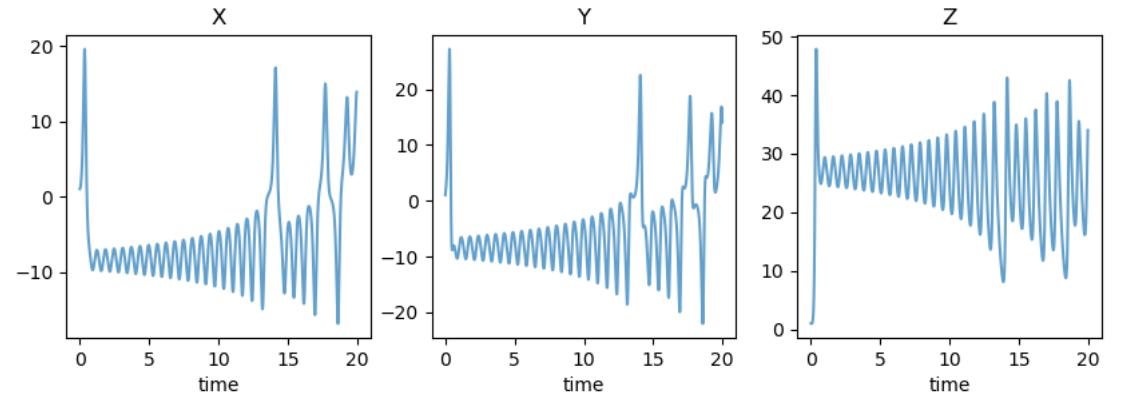
\includegraphics[width=0.8\textwidth]{img/xyz.png}
    \caption{Визуализация численного моделирования аттрактора Лоренца ($xyz$)}
    \label{fig:xyz}
\end{figure}


\subsection{Водяное колесо Лоренца}

Имеем колесо с прикреплёнными к нему корзинами, в которые льётся вода, и под действием силы тяжести колесо начинает вращаться. 
При слабом потоке оно будет стоят, а при очень сильном будет наблюдаться хаотическое движение с периодической сменой направления.

Как видно данная система, пусть и является механической и более понятной в техническом плане, представляет собой предыдущую задачу перевернутую "вверх тормашками".
	
Была предпринята попытка воссоздать систему с колесом. В качестве колеса изначально решено было взять пустую консервную банку, а по периметру её с помощью синей изоленты прикрепить пластмассовые стаканчики, с проделанными сверлом в дне отверстиями. Изначально кручение обеспечивал подвес за приклеенную к банке игрушку "спинер" , однако, в силу некачественности последней, установка сломалась, спинер развалился. 

После поломки было решено уже снизу приклеить по центру к банке чистящую липучку для одежды, которая, при смазывании маслом, тоже обеспечивала достаточно свободное вращение системы.

Под струёй воды удалось на короткое время поймать квазипериодичное (на глаз)покачивание колеса то по, то против часовой стрелки , однако данные сняты не были, так как при контрольном запуске обнаружилось, что валик разбух и мешал крутиться системе. При его устранении система теряла устойчивость.

В связи с вышеперечисленными трудностями было решено промоделировать систему с помощью \textit{Wolfram Mathematica} и довольствоваться искусственными данными.

\begin{figure}
    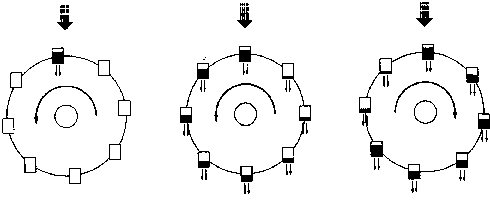
\includegraphics[width = 0.70\linewidth]{img/whaterwheel.png}
    \hspace{1cm}
    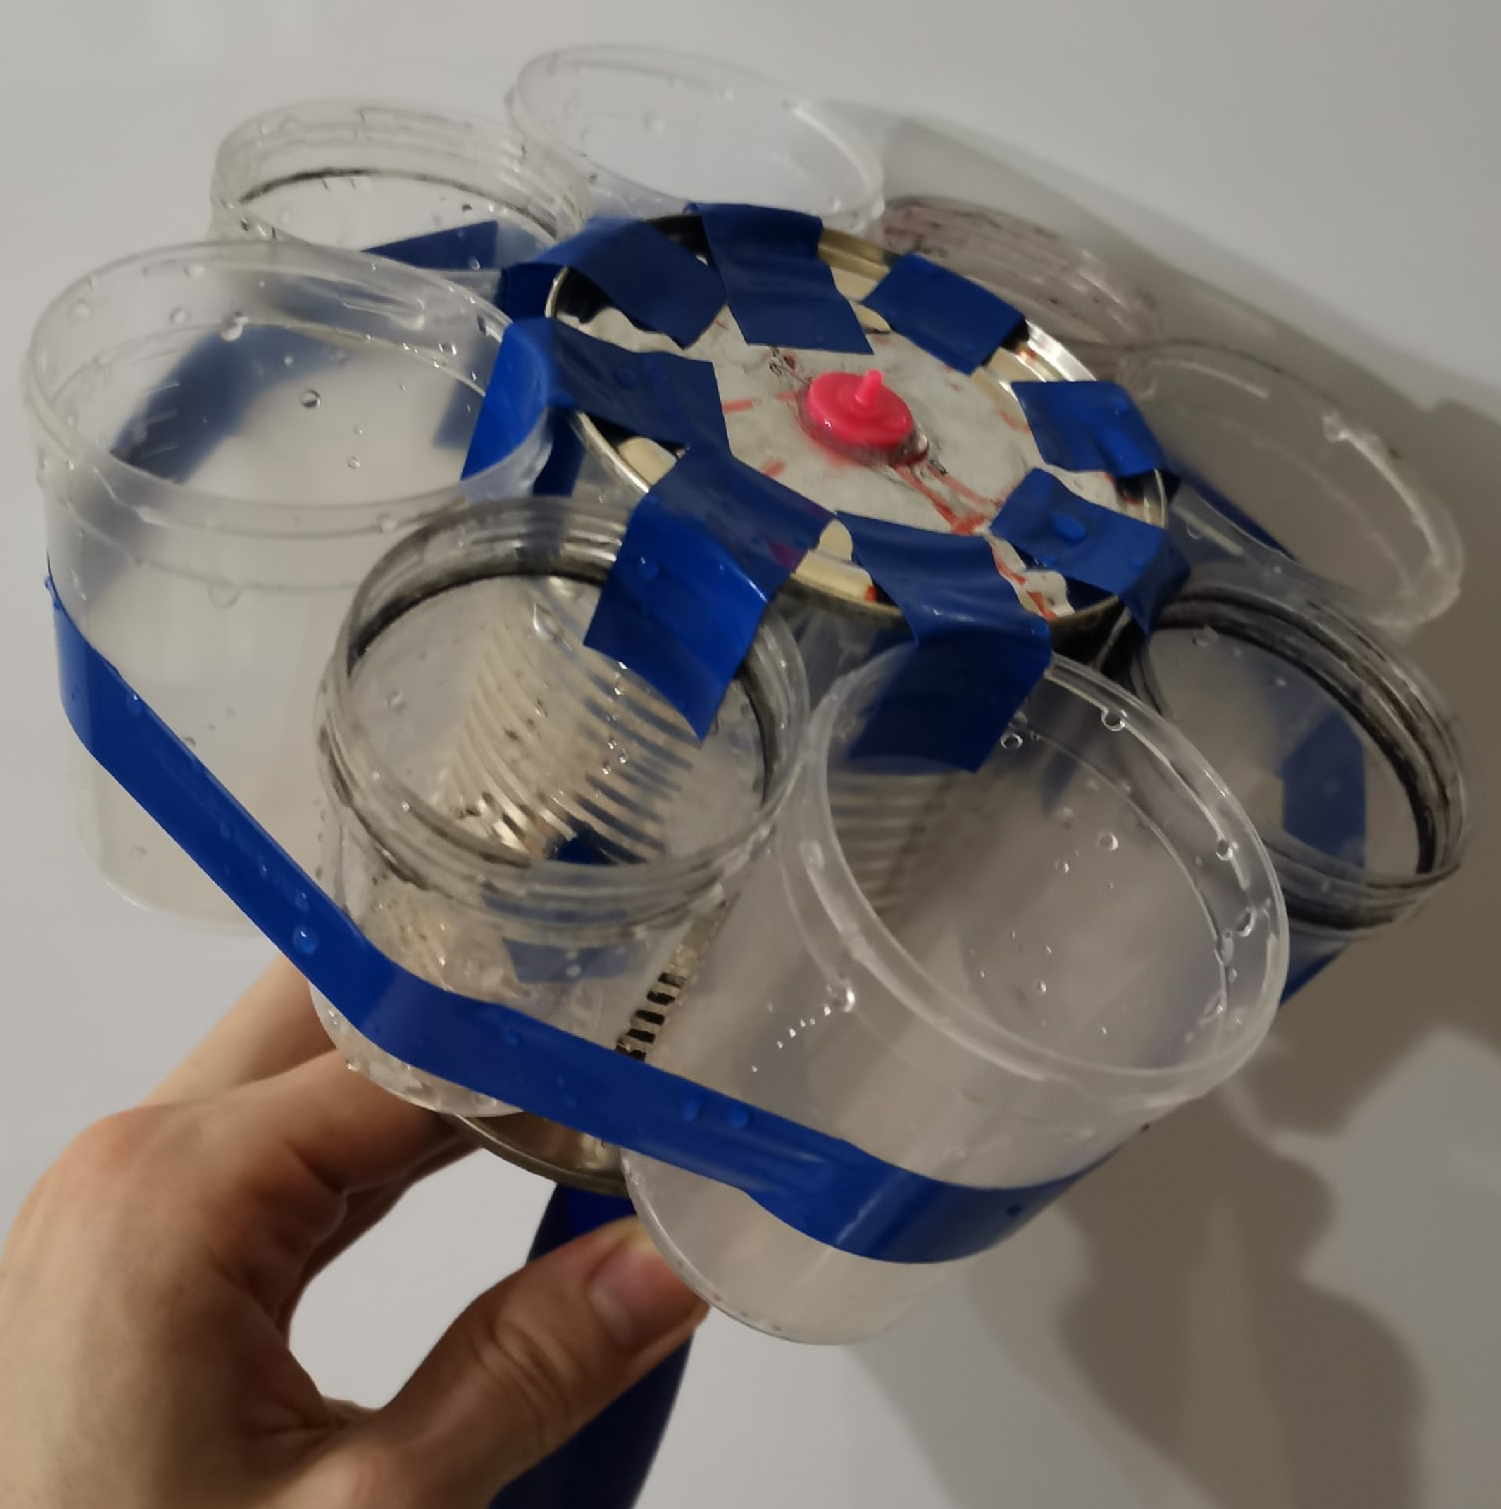
\includegraphics[width = 0.29\linewidth]{img/equipment.png}
    \caption{Схема установки и то, что получилось}
\end{figure}